\appendix
%\vspace{-3mm}
\begin{comment}
\subsection{Related Work}
\label{sec:rel}
			
\subsubsection{Peak-Constrained EV Charging Scheduling}
\label{sec:rel:peakconstrained}			
There is an extensive literature on EV scheduling problem where most of them focused on single CS \cite{Tang,Wen} and the local and global peak constraints are usually omitted or only the local peak is considered.	As discussed in Section \ref{sec:problem}, the global optimal solution cannot be obtained by separately solving the single station problems. Hence, those solutions cannot be directly applied to our problem. 
			
A scenario that local and global peak constraints exist is the case that 
scheduling is required for a charging network for multiple CSs. Studies in \cite{He,Malhotra,Moradijoz,DWang,Zeng,Shaaban} addressed charging scheduling problem in multiple CSs. The authors in~\cite{He} tackled a global EV charging scheduling problem in a system consisting of a central controller and multiple local controllers to minimize total cost. However, there is no limit on the maximum peak demand that the system can tolerate. Consequently, the peak value can be arbitrary high depending on the total demand. 
This may increase the electricity bill of large costumers substantially mainly due to very high peak demand. In addition, high EV penetration level leads to high peak which may pose danger for the grid system \cite{DWang}. Besides, the charger devices installed in the CSs have limitation on the maximum power that they can transfer in each time unit~\cite{Tesla}. We solve the issue by constraining local and global peaks. However, to meet the peak constraints, it may not be feasible to respond to all charging demands. Consequently, only a subset of EVs can be charged~\cite{Xiang}, which is captured in our integral charging model. \cite{DWang} considered a multi-microgrid system with global peak constraint where each microgrid has a CS and the goal is to minimize the operating cost of the system and the exchanged electricity between microgrids and main grid. The authors assume that charging aggregators are able to forecast required information about individual EVs which may not represent a real scenario. A similar assumption is made in \cite{Zeng,Shaaban} where the objective is to maximize total utility of EVs and aggregators in a distribution network.
			
%\rev{To be removed: In our solution, we applied a priority based selection process (based on the EVs' valuation) to respond to the demands to make sure that total peak respects the constraints. The selection process can be made based on different criteria such as the value of each charging request \cite{Lee, Xiang} or the priority.}
			
			To avoid big billing cost in peak hours, \cite{Moradijoz} proposed a solution based on genetic algorithm to find optimal capacity and location of parking lots for serving demands in peak hours with the goal of maximizing total benefit of all stations. Although authors studied the problem under multiple CS setting, their solution is not applicable to our setting when the CSs are already set up. \cite{Malhotra} employed a similar model used in this paper, where both local and global peak constraints in a charging network are considered. The objective in \cite{Malhotra} is to maximize user convenience level which is different from the aim of the problem studied in this work. More importantly, the authors solve the single-slot problem, which fails to provide a general solution taking into account EVs' arrival and departure times which are considered in our study.
%			\subsection{Peak-minimizing EV Charging Scheduling}
			As an alternative approach to control the peak, some studies directly targeted minimizing the peak \cite{Zhao, Karfopoulos}. In \cite{Zhao}, an online algorithm is developed for EV charging to minimize the peak by minimizing the impact uncertainty of renewable energies. \cite{Karfopoulos} proposed a valley filling method by leveraging V2G in peak hours. Although the peak is minimized in above works, it cannot guarantee that the minimized peak is tolerable.


\subsubsection{Scheduling Under Demand Uncertainty}
A main challenge in EV scheduling problems is to cope with demand uncertainty. Many studies including \cite{Shroff2014,Tang,WTang,Chen,Xiang,Zhao,Robu} addressed online scheduling problem with different objectives. \cite{Shroff2014,Xiang} studied the problem of maximizing social welfare considering the benefit for both users and service provider. \cite{Tang} and \cite{WTang} developed algorithms to minimize the charging price for the CS, where the proposed algorithm in \cite{Tang} is $2.39$-competitive. 
%An online algorithm developed in \cite{Chen} to optimize overall operating profit of the service provider. 
In \cite{Robu}, an online $2$-competitive algorithm is proposed for a single CS which provides incentives for the users to truthfully report their data. 

Our problem in this paper is unique from above works in different aspects. First, we study the problem in an ACN where several CSs exist. None of the above studies solve the problem under this setting. Second, the previous algorithms do not work for both integral and fractional charging models. In addition, \cite{WTang,Chen} put no limit on the charging rate of EVs which makes their solution impractical in real scenarios. Also, \cite{WTang,Tang, Shroff2014,Chen,Zhao} do not consider the peak limitation of the CS. Finally, the study in \cite{Robu} assumes that EVs are capable of getting discharged in a negligible amount of time, resulting in a $2$-competitive algorithm. However, the assumption is not realistic for EVs.
In this paper, we consider these limitations and develop online and offline algorithms for fractional and integral revenue models in an ACN and provide theoretical bounds on their performance.



%It is important to note that there is a considerable similarity between EV scheduling problem and classical job scheduling problem \cite{}. However, most algorithm developed for job scheduling problem  do not consider a limit on processing rate of the jobs. 

%\cite{Shroff2014} and \cite{Stein2012} study social welfare maximization problem while the profit of both EV owners and CS is considered.  social welfare of the EV owners \cite{Stein2012}, charging cost \cite{Tang,WTang}, and total value of fully charged EVs \cite{Azar}). In addition, \cite{WTang, Tang,Shroff2014,Zhao} do not take into account the peak limitation of CS. }
		
%\vspace{-3mm}		
\subsection{Optimal Offline algorithm for Fractional Revenue Model}
\label{sec:fopt}				
We refer the proposed algorithm as the \fcs and summarize it as Algorithm~\ref{alg:optimal-off}.
The \fcs works in two phases. In the first phase (Section~\ref{sec:ph1}), the algorithm decides on the amount of resource to be allocated to each EV within its availability window and reserves resources accordingly. In this phase, the details of allocation is not known. The actual resource allocation is done in the second phase (Section~\ref{sec:ph2}) by setting variables $y_i^t$.
		
Before discussing the details of the algorithm, we introduce some notations that facilitate our algorithm design. Let $R_i$ be the amount of resource that is reserved for EV $i$ by the \fcs and $I_{t,t'}$ as time interval $[t,t']$.
% with $t,t'\in\{1,\dots ,T\}$ which includes time slots $t,t+1,\dots ,t'$. 
Then, assuming that charging demands are sorted in non-increasing order of their unit values, $A^i_j(t,t')$ is the aggregate residual resource in interval $I_{t,t'}$ at station $j$ assuming that the reservation for EVs $1$ to $i$ is accomplished with a dummy $A^0_j(t,t')$ defined as
$$A^0_j(t,t')=(t'-t+1)\times\min \{p^\mathsf{total},p_{j}\},$$
 that indicates the available resource when no charging request is processed.
		
		\begin{defi}
			Time interval $[\delta,\delta']$ is a ``super interval'' for interval $[t,t']$ if $1\leq \delta\leq t \text{~AND~} t' \leq \delta'\leq T$.
			Moreover, $\mathcal{I}_{t,t'}$ is the set of all super intervals of interval $I_{t,t'}$ i.e., ${\mathcal{I}_{t,t'}=\{[\delta,\delta']: 1\leq \delta\leq t \text{~AND~} t'\leq \delta'\leq T\}}$.
		\end{defi}
		
%		For example, $\mathcal{I}_{1,1}=\{I_{1,1},I_{1,2},I_{1,3},\dots ,I_{1,T}\}$. 
	The number of super intervals of an interval is at most $T^2$ and at least one (for interval $[1,T]$). We now explain in detail each phase of the algorithm. 
		
		\subsubsection{Phase I-Reservation\label{sec:ph1}} In Line~\ref{algline:sort1}, the EVs are sorted in a non-increasing order of their unit values.  
%		i.e., ${v_1\slash D_1\geq v_2\slash D_2\geq\dots \geq v_n\slash D_n}$. 
		In Line~\ref{algline:setR}, the \fcs processes demand of EV $i$, picked from top of the ordered list, and sets $R_i$ as the amount to be reserved for EV $i$ which will be allocated in Phase II. In Line~\ref{algline:seta}, the residual resource of all intervals in set $\mathcal{I}_{a_i,d_i}$ decreases by $R_i$ and EV $i$ is added to the set of selected EVs.
		
			
			\begin{algorithm}[t]%\small%1
		%\footnotesize
		\caption{\fcs}
		\label{alg:optimal-off}
		\DontPrintSemicolon 
		\KwIn{$n$ EVs with their profile, local and global peak constraints $p_j, j=1,\dots ,m$ and $p^\mathsf{total}$ }
		
		\KwOut{Optimal scheduling under fractional model}
		\BlankLine
		
		Sort charging requests in non-increasing order of their unit values, i.e., $\frac{v_1}{D_1}\geq \frac{v_2}{D_2}\geq\dots \geq \frac{v_n}{D_n}$ \label{algline:sort1}
		
		%	\slash\slash\textit{\texttt{Use sorted list to process demands}}
		
		$\mathcal{L}\leftarrow \emptyset$ 	
		
		\slash\slash\textit{\texttt{Phase I}}
		
		
		\For{$i=1,\ldots, n$}{
			%\slash\slash\textit{\texttt{update demand and value}}
			
			$R_i \leftarrow \min\{D_i, \min\limits_{t,t'} A^{i-1}_{h(i)}(t,t'), \forall t,t': I_{t,t'}\in\mathcal{I}_{a_i,d_i}\}$\label{algline:setR}
			
			\If{$R_i>0$}{
				$A^{i}_{h(i)}(t,t')\leftarrow A^{i-1}_{h(i)}(t,t')-R_i, \forall t,t': [t,t']\in\mathcal{I}_{a_i,d_i}$ \label{algline:seta}\\
				$\mathcal{L}\leftarrow \mathcal{L}\cup{i}$
		}}
		\slash\slash\textit{\texttt{Phase II}}
		
		Sort EVs in $\mathcal{L}$ in increasing order of their charging flexibility i.e., $\frac{(d_i-a_i+1)k_i}{D_i}, i\in \mathcal{L}$. 
		
		%	Let $i$ be the index of $i^{th}$ EV in list $\mathcal{L}$
		
		\For{$i=1,\ldots, |\mathcal{L}|$}{
			
			Pick EV $i$ from the sorted list $\mathcal{L}$. 
			
			$\emph{feasible}\leftarrow \big(\sum_{t=a_i}^{d_i}\min\{k_i,A^{i-1}_{h(i)}(t,t)\}\big) - R_i$
			
			\If{feasible $<0$}{
				Re-allocate previously allocated EVs such that $\emph{feasible}\geq 0$
			}
		Arbitrarily allocate $R_i$ to EV $i$ in its availability window\label{algline:fcsallocate}	
		}
	\end{algorithm}


		
		\begin{lem}
			Provided that for EV $i$ we have 
			\bee
			\label{eq:ri}
			R_i\leq\min\left\{D_i, \min_{t,t'} A^{i-1}_j(t,t'), \forall t,t': I_{t,t'}\in\mathcal{I}_{a_i,d_i}\right\},
			\eee
			then there is a feasible allocation to allocate $R_i$ to EV $i$ in its availability window $[a_i,d_i]$. 
			\label{thm:R_feasible}
		\end{lem}
		
		In Eq.~\eqref{eq:ri}, the second term, i.e., $\min_{t,t'} A^{i-1}_{j}(t,t')$, indicates the minimum remaining resource in all super intervals of interval $I_{a_i,d_i}$. For $i\geq 1$, $A^i_j(a_i,d_i)$ is defined as follows:

		\begin{equation*}
			A^i_j(a_i,d_i)=\begin{cases}
			A^{i-1}_j(a_i,d_i)-R_i & j=h(i),\\
			A^{i-1}_j(a_i,d_i) & j\neq h(i).
			\end{cases} 
		\end{equation*}
		
The optimal value of $R_i, i=1,\dots ,n$ is set according to the following lemma:
		
\begin{lem}
			Given $n$ EVs sorted in a non-increasing order of the unit values, ${v_1\slash D_1\geq v_2\slash D_2\geq\dots \geq v_n\slash D_n}$, and the value of $R_i$, where $R_i$ is set after $R_{i-1}, i=2,\dots ,n$ by Eq.~\eqref{eq:ri}, then, 
$$R_i = \min\left\{D_i, \min_{t,t'} A^{i-1}_{h(i)}(t,t'), \forall t,t':I_{t,t'}\in\mathcal{I}_{a_i,d_i}\right\},\forall i,$$
 is the optimal value for $R_i$. 
\label{thm:R_star}
\end{lem}
			
			\subsubsection{Phase II- Allocation\label{sec:ph2}} Lemma~\ref{thm:R_feasible} shows that there is a feasible scheduling to allocate the reserved resources.
However, despite its feasibility, it is not straightforward to find such scheduling. For example, assume that for EV $i$ it is set that $R_i=10$ and $k_i=4$. It is possible that all available resources are concentrated in a single time slot but EV $i$ cannot use more than $4$ kWh of it. In this situation, the previously allocated resources in interval $I_{a_i,d_i}$ should be re-allocated such that the concentrated resources are \emph{dispersed} and we have $\sum_{t=a_i}^{d_i}\sigma_t \geq R_i$ where $\sigma_t =\min\{k_i,A^{i-1}_{h(i)}(t,t)\}$ is the maximum resource that can be allocated to EV $i$ at time slot $t$. Since the total amount of allocated resource does not change in the interval, such dispersion is possible and can be done by a simple algorithm in which allocates $\min\{k_i,A^{i-1}_{h(i)}(t,t)\}$ starting from time slot $t=a_i$ until $R_i$ units is allocated. To further reduce the peak of the system, we will develop \sa\ algorithm (See Section \ref{sec:integral}) which acts more intelligent so that Line \ref{algline:fcsallocate} of the \fcs can be replaced by ``Run \sa$(i,R_i)$''.
  

			
			\begin{thm}
				\label{cor:1}
				\fcs is an optimal solution under fractional revenue model.
			\end{thm}

The following theorem characterizes the complexity of \fcs.
			
			\begin{thm}
				\label{thm:complexity}
				The time complexity of \fcs algorithm is $O(n^2T+nT^2)$ where $n$ is the number of EVs and $T$ is number of time slots.
			\end{thm}



\vspace{-3mm}

\subsection{OLP algorithm}	
\label{app:olp}

The Online Linear Program (OLP) \cite{lee2016adaptive} is a greedy algorithm that works as follows:
(i) at $t=1$ compute the optimal solution (e.g., by a solver) for the current set of EVs assuming that there will be no further arrival. (ii) use the solution until there is a new arrival. (iii) when an EV arrives, construct and solve a new problem by considering the new arrivals and the remaining demand of previously arrived EVs which are still active. (iv) go back to (ii).

The original OLP algorithm which is implemented in Caltech ACN works only for integral revenue model and under different cost functions including the revenue of the charging stations, which is the case of our study. In this paper, we implemented the algorithm for both integral and fractional model. The difference between the two versions is in the constraint set of the optimization problem that should be solved such that in integral model, the total amount of resource that an EV receives can only be equal to zero or its demand while in fractional model it can be any non-negative value less than or equal to the demand. 

\end{comment}

%\vspace{-3mm}
\subsection{Details of the \rc($i$)}
\label{sec:rc}
		Before giving the details of \rc($i$), we first explain the intuition behind this algorithm. 
		 Note that if in the scheduling problem we set $T=1, m=1, k_i=p^\mathsf{total}, a_i=d_i=1\ \forall i$, then the problem is equal to the well-known $0$-$1$ knapsack problem~\cite{approx}. In the knapsack problem, a widely used greedy approach sorts items based on their unit values and selects items accordingly. It turns out that in this approach the approximation factor can be arbitrarily bad. For example, consider a knapsack problem with two items with $v_1=2, v_2=p^\mathsf{total}, D_1=1$, and  $D_2=p^\mathsf{total}$. Given these values we have $v_1\slash D_1>v_2\slash D_2$. To maximize total value of selected items, the optimal solution chooses item $2$ while greedy algorithm selects item $1$ which results in a worst-case approximation factor of ${c \slash \opt}$ in general where $c$ is a constant (in this example $c=2$). To resolve it, one approach is to \emph{re-consider} unselected items after running greedy algorithm and replace some selected items in the knapsack with unselected ones and then check whether the result is improved or not. In a simple case, only the largest unselected item can be examined which makes a significant theoretical improvement by providing a worst case approximation factor of $\opt\slash 2$.
	 
\ics algorithm leverages the same idea but using a more intelligent replacing method called \rc($i$). \rc($i$) is called on every unselected EV $i$. It tries to find some selected EVs that if they are replaced by EV $i$, total revenue from the selected EVs increases. 
%%%When \ics calls \rc($i$) on all unselected EVs, an improvement in total revenue of final selected EVs is expected. 
%This is confirmed by the simulation results in Section~\ref{sec:simul}.
	
	
%\vspace{-3mm}
%%end{comment}			
			
\subsection{Proof of Lemma~\ref{thm:R_feasible}}
			\label{app:2}
			We prove the theorem by induction. 
			
			\textbf{Base case}: When $n=1$, there is only one EV that can be easily scheduled in its interval since all charging profiles represent a feasible demand and all resources are free.
			
			\textbf{Induction step}: Let $k\in\mathbb{Z}^+$ is given and the claim is true for $n=k$ i.e., EVs $1,\dots , k$ can be feasibly scheduled to receive their reserved resources. Now let $n=k+1$. We claim that EV $k+1$ can be feasibly scheduled in its interval. To prove, assume that this claim does not hold. Therefore, there should be at least one interval say $I_{t,t'}$ such that $A^{k+1}_{h(k+1)}(t,t')<0$ and $A^{k}_{h(k+1)}(t,t')\geq 0$. Then, one of the following cases holds: \textit{a})  $I_{t,t'}\notin\mathcal{I}_{a_{k+1},d_{k+1}}$ and \textit{b})  $I_{t,t'}\in\mathcal{I}_{a_{k+1},d_{k+1}}$. 
			%Moreover, we have $R_{k+1}=A^{k}_{a_{k+1},d_{k+1}}-A^{k+1}_{a_{k+1},d_{k+1}}$.
			
			In case \textit{a}, since $I_{t,t'}\notin\mathcal{I}_{a_{k+1},d_{k+1}}$, reserving resources in interval $I_{a_{k+1},d_{k+1}}$ does not affect remaining resource in $I_{t,t'}$. Therefore, we have $A^{k+1}_{h(k+1)}(t,t')=A^{k}_{h(k+1)}(t,t')\geq 0$. 
			
			In case \textit{b}, according to Eq. (\ref{eq:ri}), we have $R_{k+1}\leq A^{k}_{h(k+1)}(t,t')$. Also, $A^{k+1}_{h(k+1)}(t,t')=A^{k}_{h(k+1)}(t,t')-R_{k+1}$ which gives $A^{k}_{h(k+1)}(t,t')\geq 0$.
			
			Consequently, in both cases $A^{k}_{h(k+1)}(t,t')\geq 0$ which is a contradiction. Therefore, the original claim holds.
			
%\vspace{-3mm}
\subsection{Proof of Lemma~\ref{thm:R_star}}
			\label{app:3}
			By induction.
			
			\textbf{Base case:} When $n=1$, the claim holds since $R_i>\min\{D_i, \min_{t,t'} A^{i-1}_{h(i)}(t,t'), \forall t,t': [t,t']\in\mathcal{I}_{a_i,d_i}\}$ is not feasible and the gain is maximized with maximum value of $R_i$ i.e., $R_i=\min\{D_i, \min_{t,t'} A^{i-1}_{h(i)}(t,t'), \forall t,t': [t,t']\in\mathcal{I}_{a_i,d_i}\}$.
			
			\textbf{Induction step:} Assume the claim holds for $n=k, k>1$ i.e., $R_i^\star=\min\{D_i, \min_{t,t'} A^{i-1}_{h(i)}(t,t'), \forall t,t': [t,t']\in\mathcal{I}_{a_i,d_i}\}$, is the optimal value for $R_i, i=1,\dots ,k$. Now let $n=k+1$. We claim that $R^\star  _{k+1}=\Gamma$ where  $\Gamma =\min\{D_{k+1}, \min_{t,t'} A^{k}_{h(i)}(t,t'), \forall t,t': (t,t')\in\mathcal{I}_{a_{k+1},d_{k+1}}\}$. To prove, assume $\Gamma$ is not the optimal value of $R_{k+1}$. Therefore, since according to the definition of $R_{k+1}$ it always holds that $R _{k+1}\leq\Gamma$ thus, $R^\star _{k+1}<\Gamma$ and the amount of resource to be reserved for EV $i$ is decreased by $\Gamma - R^\star _{k+1}$. This amount, can be only assigned to EVs $k+2$ to $n$ since $R_i$ is set to its maximum value for $i=1,\dots , k$. However, having $v_{k+1}\slash D_{k+1}\geq v_{i}\slash D_{i}, i=k+2,\dots ,n$ the optimal total revenue can be increased by setting $R_{k+1}=\Gamma$ which is a contradiction.
	
	
\subsection{Proof of Theorem~\ref{thm:focscompetitive}}
	\label{app:focscompetitive}
	
	We first prove the theorem for single station scenario and then extend it to multiple stations. From (\ref{eq:optdist}), (\ref{eq:lg}), and (\ref{eq:ALG}) we obtain the following result
\begin{equation}
\label{eq:compsingle}
\opt-\alg\leq \sum_{i=1}^n\sum_{t=1}^Tg_{i,t}\leq\alg,
\end{equation}
hence, $\opt\leq 2\alg$. 

In multi-station setting, the difference with the previous case is that when $\Delta_{i}^t>0, i\in\{1,\dots,n\}$, then \focs may allocate the difference $\Delta_{i}^t$ to one or multiple EVs in any CS that might not be $h(i)$. However, the inequality $l_{i,t}\leq g_{i,t}$ is still valid as \focs is centralized and uses a single sorted list for all EVs. Using similar deductions as in the single station setting, it is easy to verify that the competitive ratio of $2$ is preserved.
		
		%\subsection{Proof of Theorem~\ref{thm:focscomplexity}}
			%\label{app:focscomplexity}
			
	%The complexity of the algorithm is identified by sorting operation at each time slot which dominates the $O(n)$ cost of the ``for'' loop. Therefore, the total time complexity is $O(nT\log n)$.	
	

		
\subsection{Proof of Theorem~\ref{thm:approx}}
			\label{app:1}
			Without loss of generality we assume that $a_i=1, \forall i$, however, the proof holds for any other constant value for arrival time. We sum up all costs of covering dual constraints and then provide a bound for it. 
			
			Each EV is either selected or not selected. For the unselected EVs, $\sum_{j=1}^m \sum_{t=1}^T p_j\beta (t)$ determines the cost. When \bc($i$) is running as a result of charging request disapproval of EV $i$, for any previously accepted request $i'$ the algorithm sets $\Phi_{i'}(t)$ to a value proportional to $y_{i'}^t$ for $t\leq R(d_i)$ (Line 8 of \bc($i$) algorithm). The followings are proved in \cite{Jain} for a single station $h(i')=h(i)=j$:
			
			\begin{equation}
				\sum_{i'=1}^n \sum_{t=1}^{d_{j}} \Phi_{i'}(t) \leq \bigg[ \frac{p_j}{p_j-q_j}.\frac{s}{s-1} \bigg].\sum_{i'=1}^n v_{i'}
				\label{EqCharge}
			\end{equation} 
			
			\begin{equation}
				\sum_{t=1}^T p_j\beta (t)\leq \sum_{i'=1}^n \sum_{t=1}^{d_{j}} \Phi_{i'}(t).
				\label{EqBound}
			\end{equation}
			
			
			For $m$ CSs, we can obtain the following inequality based on (\ref{EqCharge}) and (\ref{EqBound}),
			
			\begin{align}
				\sum_{j=1}^m \sum_{t=1}^T p_j\beta (t)&\leq \sum_{j=1}^m \Big( \frac{p_j}{p_j-q_j}.\frac{s}{s-1}\sum_{i: h(i)=j}v_{i}\Big)\label{EqMS}.
			\end{align}
			
			Now for notational convenience let's define $A_j, B_j$ and $C$ as follows:
			
			\begin{align} 
				A_j&=\frac{p_j}{p_j-q_j}.\frac{s}{s-1},\nonumber\\ 
				B_j&=\sum_{i:h(i)=j}v_i,\nonumber\\ 
				C&=\sum_{j=1}^m B_j=\sum_{i=1}^n v_i\nonumber. 
			\end{align}
			
			We can write the right hand side of Eq.~\eqref{EqMS} as follows:
			
			\begin{align}
				\sum_{j=1}^m A_jB_j&=\sum_{j=1}^m \Big[ A_j\big(C-\sum_{i:h(i)\neq j}B_{h(i)}\big)\Big]\nonumber\\
				&=\sum_{j=1}^m A_jC - \sum_{j=1}^m \Big[ A_j\sum_{i:h(i)\neq j}B_{h(i)} \Big]\nonumber\\
				&=\sum_{j=1}^m A_jC - \sum_{j=1}^m \Big[ A_j\big( C-B_{j}\big) \Big]\nonumber\\
				&\leq\sum_{j=1}^m A_jC- \sum_{j=1}^m \Big[ A_j\big( C-\max_j \{B_j\} \big) \Big]\nonumber\\
				&=\max_{j}\{B_{j}\} \sum_{j=1}^m A_j\label{Eqabf}.
			\end{align}
			From (\ref{EqMS}) and (\ref{Eqabf}) we get
			\begin{align}
				\sum_{j=1}^m \sum_{t=1}^T p_j\beta (t)&\leq \max_{j}\{B_{j}\}\sum_{j=1}^m{\frac{p_j}{p_j - q_j}}.\frac{s}{s-1}
			\end{align}
			
			
			For the selected EVs, the covering cost is determined by the term $\sum_{i} D_i\alpha _i$ in the dual objective which equals to $\sum_{i\in \mathcal{S}} v_i$ where $\mathcal{S}$ is the set of selected EVs. Therefore, the total cost of covering dual constraints equals to 
			\begin{align}
				&\Lambda =  \sum_{i\in \mathcal{S}}v_i + \max_{j}\{B_{j}\}\sum_{j=1}^{m}{\frac{p_j}{p_j-q_j}}.\frac{s}{s-1}\nonumber\\
				&\leq \sum_{i\in \mathcal{S}}v_i + \sum_{i\in \mathcal{S}}v_i\sum_{j=1}^{m}{\frac{p_j}{p_j-q_j}}.\frac{s}{s-1}\nonumber\\
				&=\Big[ 1+\sum_{j=1}^m{\frac{p_j}{p_j-q_j}}.\frac{s}{s-1}\Big] \sum_{i\in \mathcal{S}}v_i\label{Eq:bound}
			\end{align}
			Given that the primal value obtained from \ics is 
			${\Gamma = \sum_{i\in \mathcal{S}}v_i}$, we get 
			\bee
			\Lambda \leq \Big[ 1+\sum_{j=1}^m{\frac{p_j}{p_j-q_j}}.\frac{s}{s-1}\Big] \Gamma.
			\eee
			Finally, considering the fact that $\Lambda\geq\opt$, we conclude that \ics is $\Big[1+\sum_{j=1}^m{\frac{p_j}{p_j-q_j}}.\frac{s}{s-1}\Big]$-approximation.
			
%\subsection{Proof of Theorem~\ref{thm:ics_complexity}}	
%\label{app:ics_complexity}	

%\ics starts by sorting demands which costs $O(n\log n)$. The inner ``for'' loop in Line $5$ costs $O(nT)$ and running \sa($i,D_i$) and \bc($i$) costs $O(T\log T)$ and $O(nT)$, respectively. Therefore, the total cost of outer ``for'' loop (Line $4$) equals to $O(nT\log T+n^2T)$. The complexity of \rc($i$) called in the ``for'' loop in Line $14$ is $O(nT)$. Therefore, the total cost is $O(nT\log T+n^2T)$.		

\vspace{-3mm}
\subsection{Proof of Theorem~\ref{thm:iocscompetitive}}	
\label{app:iocscompetitive}	

In the worst case $b=T$ i.e., there are $T$ groups where at each time slot, a group of EVs arrive. Observe that 

$$\opt\leq\rho\Gamma_{\mathcal{A},\mathcal{R}^1}+\dots +\rho\Gamma_{\mathcal{A},\mathcal{R}^T}.$$ 

Put it simply, the increase in optimal gain at each time slot is at most equal to maximum gain that can be obtained from arrived EVs at time slot $t$. Moreover, according to the \iocs, the gain of the algorithm obtained from set of active jobs at each time slot $t$, $\Gamma_{\iocs}^t$, is as follows: $$\Gamma_{\iocs}^t=\max\{\widehat{\Gamma}_{\mathcal{A},\mathcal{R}^t},\Gamma_{\mathcal{A},\mathcal{M}^t}\}.$$ Therefore, 

$$\Gamma_{\mathcal{A},\mathcal{R}^t}\leq \Gamma_{\iocs}^t, t=1, \dots ,T$$

Thus, $\opt\leq T\Big(1+\frac{p}{p-q}\frac{s}{s-1}\Big).$ If $b<T$, we can obtain $\opt\leq b\Big(1+\frac{p}{p-q}\frac{s}{s-1}\Big)$ by the same analysis.

%It is easy to verify that in a single station scenario, the competitive ratio of \iocs is at most $b\rho$ where $\rho$ is the competitive ratio of algorithm $\mathcal{A}$. As an example, if EVs arrive in two groups and $\mathcal{A}$ is \ics, then \iocs is $2+\frac{2C}{C-k}\frac{s}{s-1}$-competitive. For the proof, 

%\subsection{Proof of Theorem~\ref{thm:iocscomplexity}}	
%\label{app:iocscomplexity}

	%The time complexity of \iocs is determined by the cost of algorithm $\mathcal{A}$ that it calls at each time slot. Assuming that $\mathcal{A}$ is \ics, the complexity of \iocs in a single time slot is $O(n^2)$, according to Theorem $\ref{thm:ics_complexity}$. Therefore, the complexity of \iocs is $O(n^2T)$.	
	
%***********************************************


\vspace{-3mm}		
		
				
%\vspace{-3mm}			
\subsection{Proof of Theorem~\ref{cor:1}}
			\label{app:4}
			By utilizing Lemma \ref{thm:R_star}, \fcs sets $R_i$ to its optimal value for EV $i, i=1,\dots ,n$. Based on Theorem \ref{thm:R_feasible}, since it is feasible to allocate $R_i$ to EV $i, i=1,\dots ,n$, the total gain by \fcs is optimal. 
			
\vspace{-3mm}
\subsection{Proof of Theorem~\ref{thm:complexity}}
			\label{app:5}
			The algorithm starts by sorting the charging profiles which costs $O(n\log n)$. Then, in the first 
			``for'' loop in Lines $4-8$, the algorithm calculates $R_i$ for $i=1,\dots ,n$. This requires us to check that for each EV $i$, there are enough available resources in all time intervals in the set $\mathcal{I}_{a_i,d_i}$. By definition, number of these times slots is $(T-d_i+1)a_i$ which is $O(T^2)$ and their length varies from $1$ to $T$. Therefore, the complexity of the first ``for'' is $O(nT^2)$. Finally, in the second ``for'' loop where the algorithm makes re-allocations, it should check all previously allocated EVs in their availability interval which can be done in $O(n^2T)$ and dominates the cost of sub procedure \sa. Therefore, the total cost is $O(n^2T+nT^2)$. 
			
\vspace{-3mm}


\begin{comment}
\subsection{The Impact of Slackness Parameter}
\label{sec:sim:slack}
This section discusses on the benefits and disadvantages that can be brought by using slackness parameter. To give the charging scheduler more flexibility, a slackness parameter $s\geq 1$ is used and set by the system designer. 
Recall that charging profile of EV $i$ is feasible if $D_i\leq k_i\frac{d_i-a_i+1}{s}$ holds. Since users have no control on the slackness parameter and the maximum charging rate, they must adjust their demand and availability according to the imposed slackness value. Based on the charging profile feasibility equation, when the slackness value increases users have two choices to react: (i) decrease the demand and depart at the desired deadline or, (ii) extend the deadline and receive the desired demand. In the remaining of this section, we investigate the effects of either case by simulation. To have a clear picture of effects caused by slackness parameter, we generated $100$ initial charging profiles $\langle a_i,d_i,v_i,D_i,k_i\rangle$ for $100$ EVs randomly and uniformly chosen from $10$ different models in Table \ref{tb:models} such that the initial profiles are set up assuming that the CS allows the charging operations to be finished at earliest possible time (i.e., $\frac{D_i}{k_i}$) with $s=1$. For each EV, its demand is randomly chosen from $25\%$ to $100\%$ of its battery capacity and departure in  interval $[a_i+\frac{sD_i}{k_i},T]$, where $a_i+\frac{sD_i}{k_i}$ is the earliest feasible deadline. Then, the EVs are uniformly assigned to $4$ CSs and should choose one of the above strategies to submit a feasible demand according to imposed slackness. 

\begin{figure}[t]
\centering
				\begin{subfigure}[b]{0.236\textwidth}
					\begin{center}
						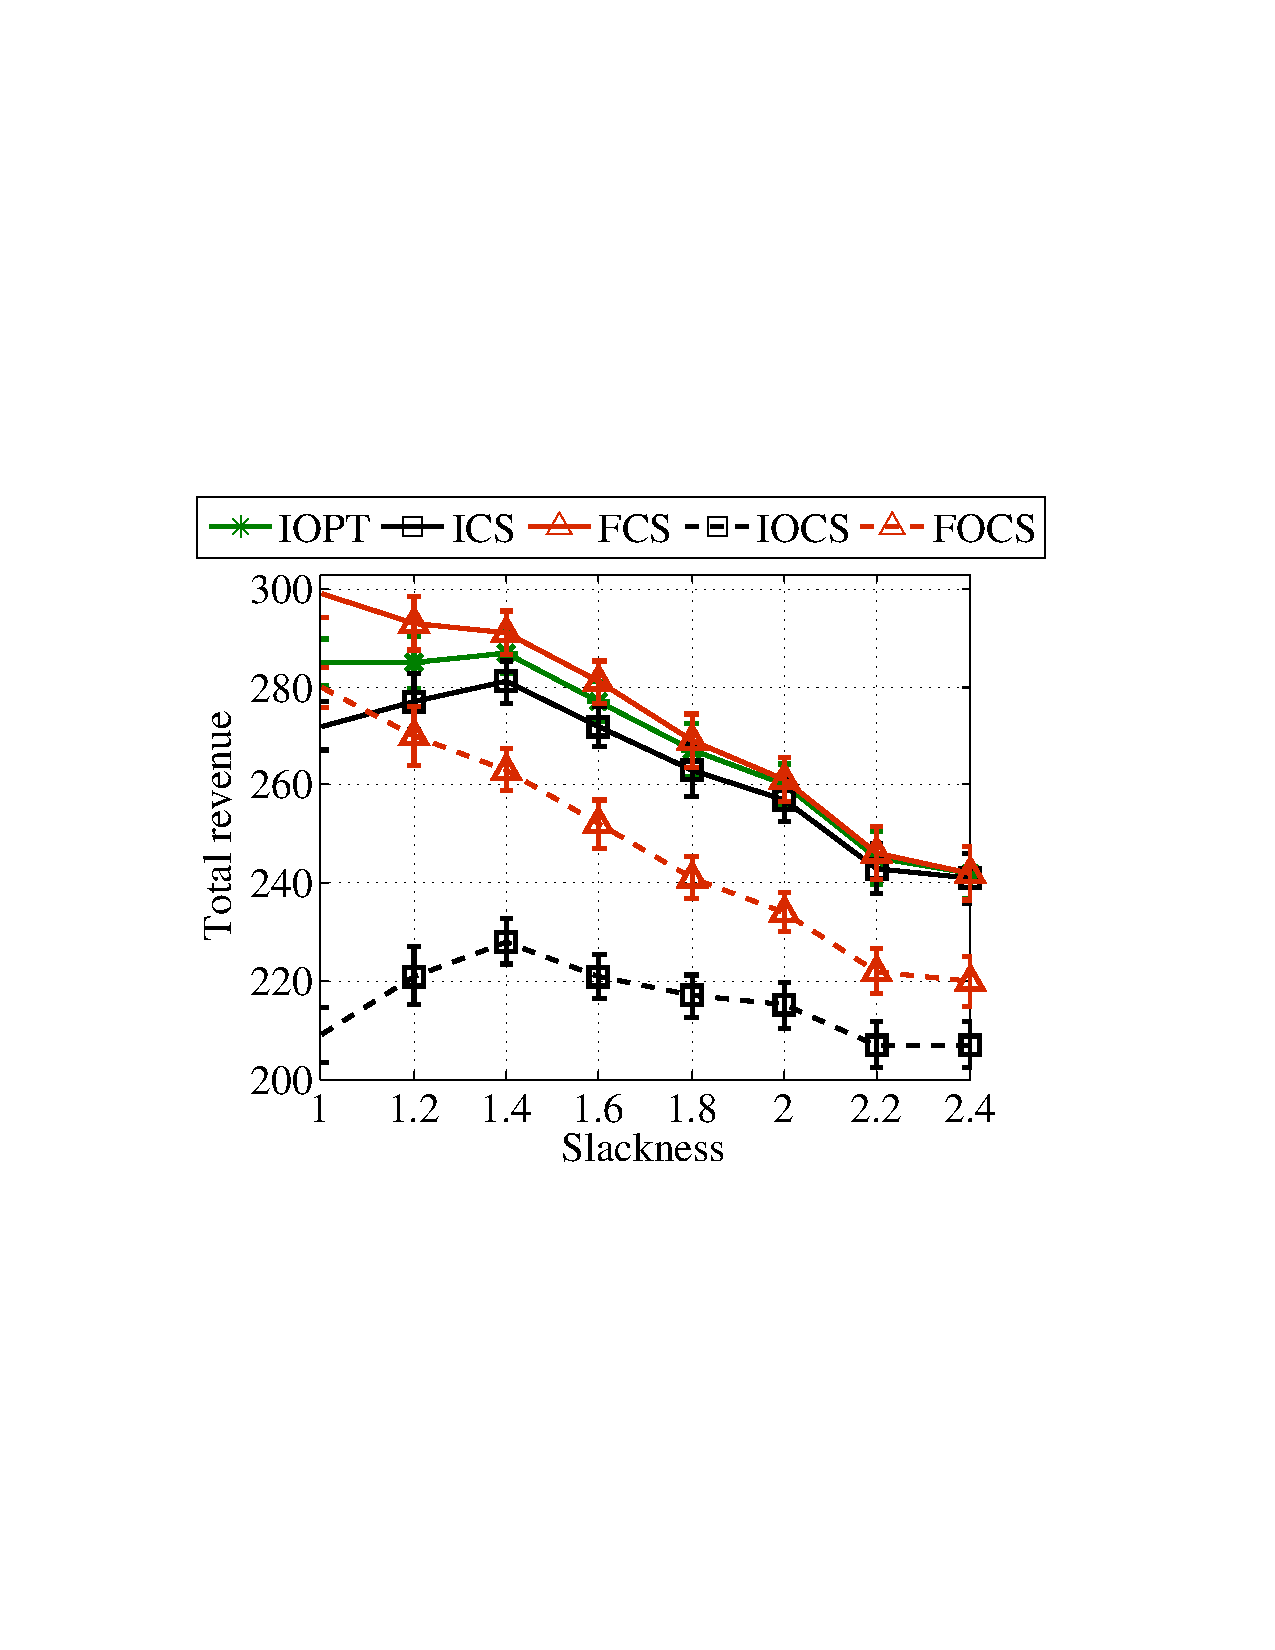
\includegraphics[width=\textwidth]{v-s-method1.pdf}
						\caption{Total revenue (\$)}
						\label{fig:v-s-method1}
					\end{center}
				\end{subfigure}%				
				\begin{subfigure}[b]{0.236\textwidth}
					\begin{center}
						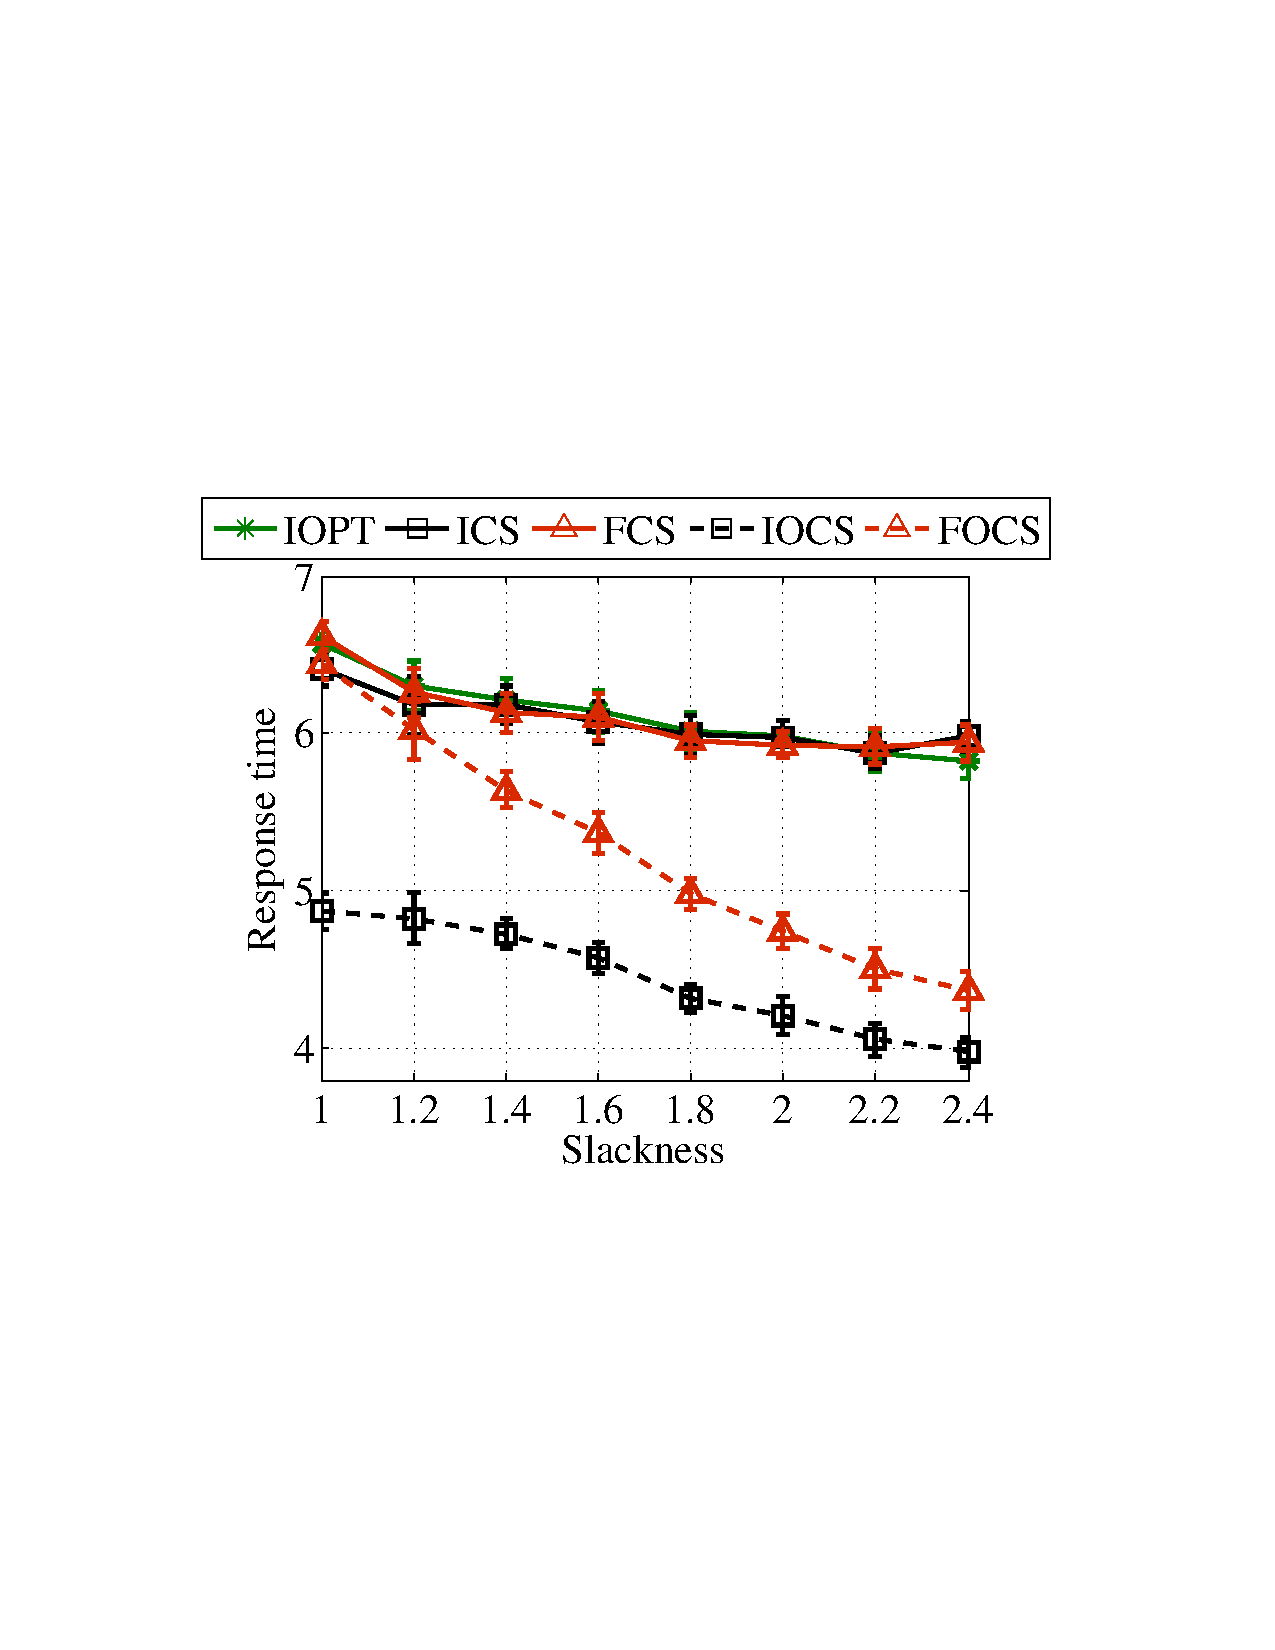
\includegraphics[width=\textwidth]{rt-s-method1.pdf}
						\caption{Response time (hr))}
						\label{fig:rt-s-method1}
					\end{center}
				\end{subfigure}%  
\caption{The impact of slackness parameter on total revenue and response time when users react by adjusting their demand.} 
\label{fig:slackness1}
\end{figure}
%\vspace{-1cm}

\begin{figure}[t]	
\vspace{-2mm}
\centering
							\begin{subfigure}[b]{0.236\textwidth}
								\begin{center}
									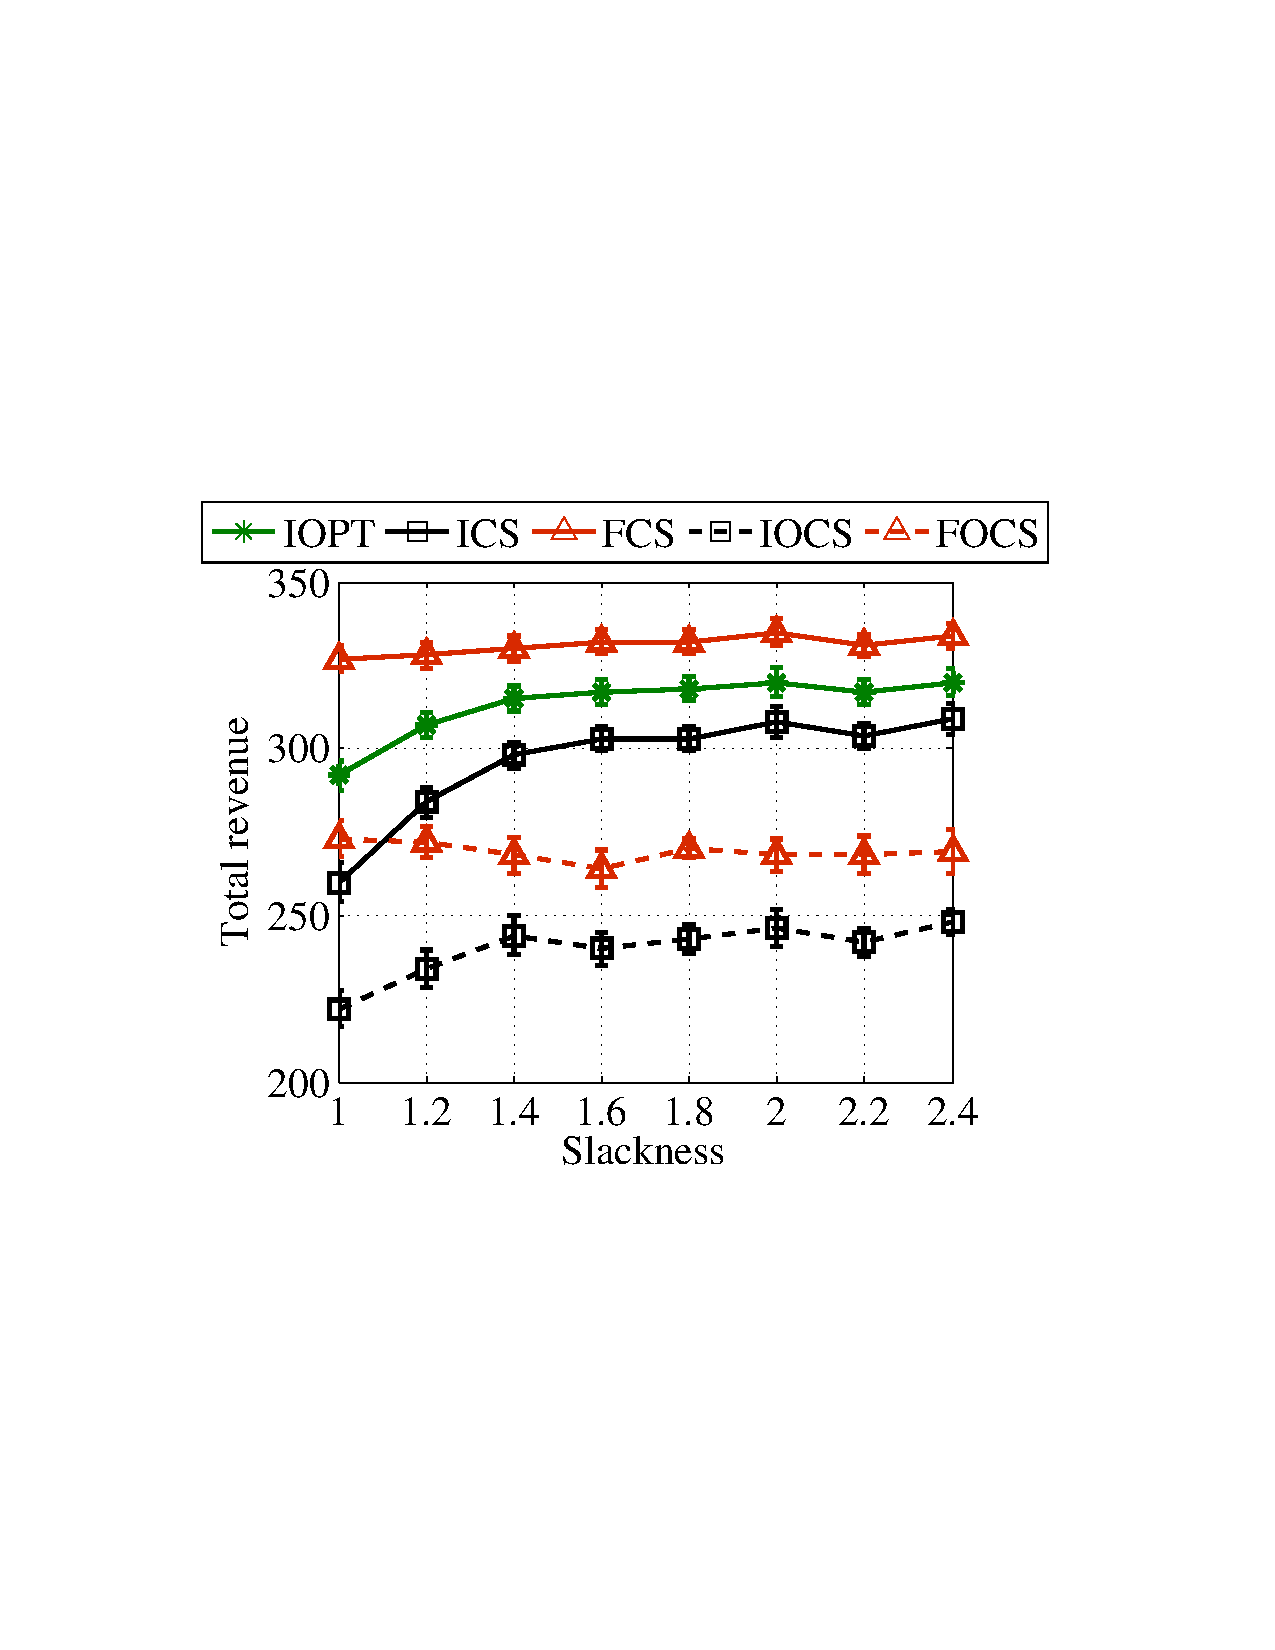
\includegraphics[width=\textwidth]{v-s-method2.pdf}
									\caption{Total revenue (\$)}
									\label{fig:v-s-method2}
								\end{center}
							\end{subfigure}%
							\hspace{1mm}
							\begin{subfigure}[b]{0.236\textwidth}
								\begin{center}
									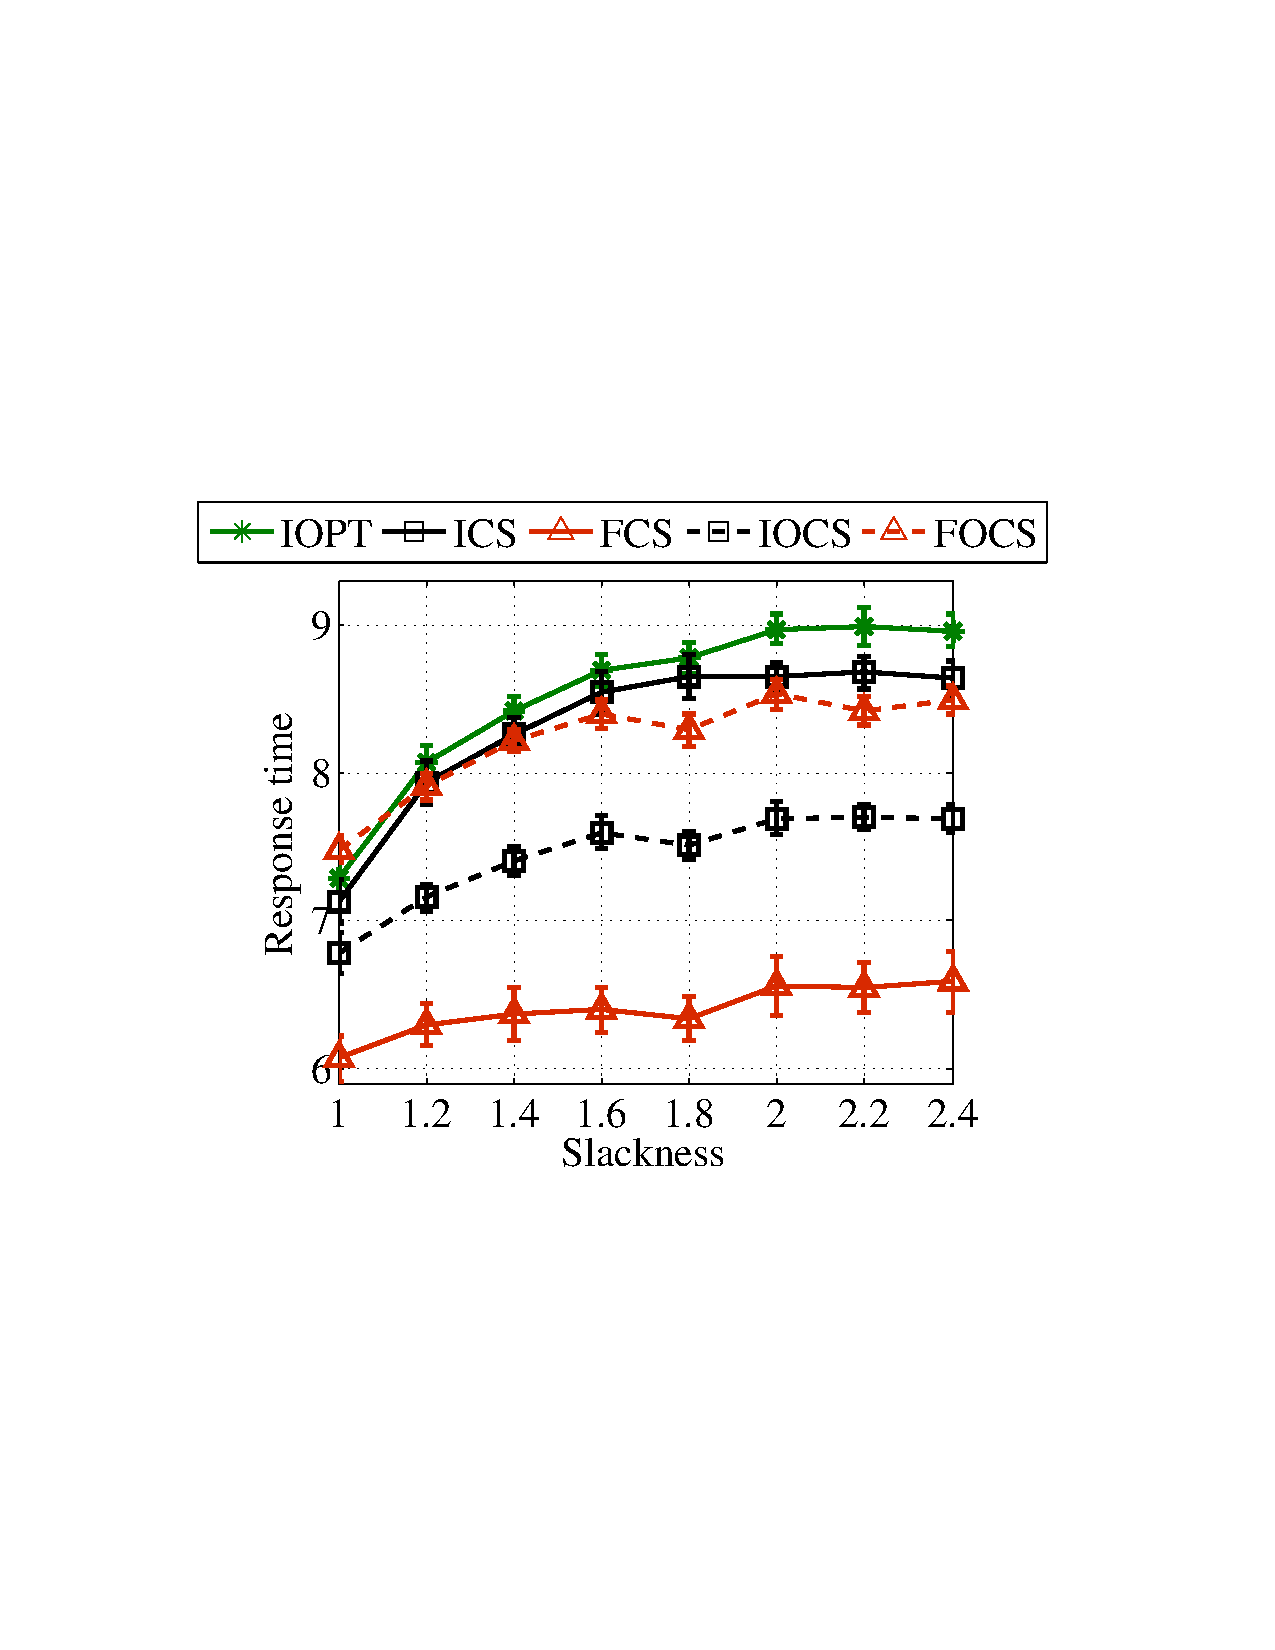
\includegraphics[width=\textwidth]{rt-s-method2.pdf}
									\caption{Response time (hr)}
									\label{fig:rt-s-method2}
								\end{center}
							\end{subfigure}% 
							
\caption{The impact of slackness parameter on total revenue and response time when users react by adjusting their deadline.} 
\label{fig:slackness2}
\end{figure}
			
\subsubsection{Case I- Adjusting Demands}
In this case, if the initial charging profile of an EV does not reflect a feasible charging request based on the slackness parameter, the EV owner decreases its demand so it will be able to leave CS at its initial desired deadline. Note that the valuation of EVs decreases proportionally, as well. Fig.~\ref{fig:slackness1} depicts the result under this policy applied by users. As it can be seen in Fig. \ref{fig:v-s-method1} and Fig. \ref{fig:rt-s-method1}, the general trend is that both total revenue and average response time decrease when slackness value increases. This is justifiable based on users reaction. When users decrease their demand, less electricity is sold which results in less revenue. When total demand decreases, charging can be finished in shorter time which decreases response time. Therefore, if users choose the first policy (adjusting their demand), total revenue degrades while response time improves. Notice that for the algorithms working under integral revenue model (i.e., \textsc{iOPT}, \ics and \iocs) the total revenue increases with slackness parameter at first (when $s$ grows from $1$ to $1.4$) but then it decreases when the slackness increases more (for $s>1.4$). 
In our view, this happens because increasing the slackness in integral revenue model makes it possible to \emph{fully} charge more EVs at the beginning as the demands decrease. However, when the slackness increases more, it results in opposite effect because the valuation of demands decreases along with the demands' size.	
			\subsubsection{Case II- Adjusting Deadlines}
			In this case, we assume that users are reluctant to decrease their desired demands. Instead, they can extend their departure. In Fig.~\ref{fig:slackness2} it can be observed that under this behavior of the users, the results are opposite as compared to the previous case (Fig.~\ref{fig:slackness1}). When deadlines are extended without demand decrement, the scheduler has more chance to compliance the demands through improved scheduling flexibility. Consequently, the total revenue increases by increasing slackness value while average response time degrades. 
%%Also observe the behavior of the online algorithms (i.e., \iocs and \focs) where both total revenue and response time decrease after a specific point that is $s=1.8$. When deadlines extend, more EVs have the opportunity of getting charged	
%					
We can conclude that when total revenue is more important than the response time, the CS should impose small values of slackness for users that apply the policy of the first case and impose higher values of slackness for the users that apply the second policy. The conclusion is reverse for the case that the objective is to have lower response times. 

			%In fact, the slackness parameter controls the maximum demand or earliest deadline that an EV can submit to the system. Remember that demands are in interval $[\textrm{min}\{\frac{d_i-a_i}{sk_i},U_i\},U_i]$ for EV $i$ meaning that the maximum demand that an EV can submit decreases by increasing slackness parameter. A reduction in total demand result in lower charging costs. Therefore, the total revenue decreases with higher values of parameter $s$ as in Fig. \ref{fig:v-s}. 
			%Also, the percentage of EVs that received all of their requested demand increases based on the same fact. The main goal of this simulation is to observe that obtained theoretical result on approximation ratio is confirmed as optimality gap of the SCS algorithm reduces by increasing $s$ in Fig. \ref{fig:v-s}. 

\end{comment}